% This file was created with tikzplotlib v0.10.1.
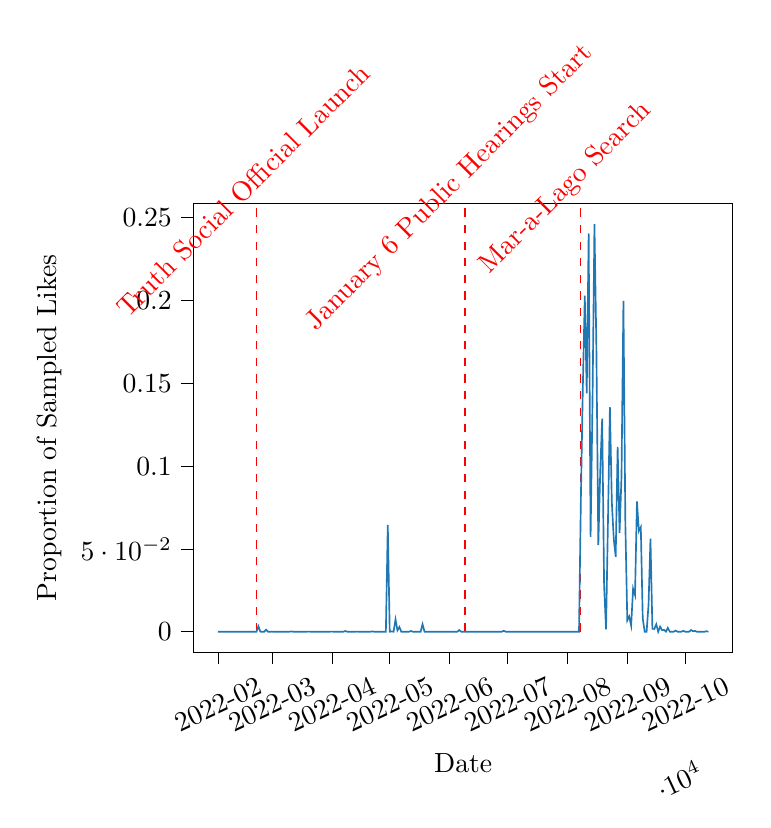
\begin{tikzpicture}

\definecolor{darkgray176}{RGB}{176,176,176}
\definecolor{steelblue31119180}{RGB}{31,119,180}

\begin{axis}[
tick align=outside,
tick pos=left,
x grid style={darkgray176},
xmin=19011.3, xmax=19290.7,
xlabel={Date},
xticklabel style={rotate=25.0},
ylabel={Proportion of Sampled Likes},
clip=false,
xtick style={color=black},
xtick={19024,19052,19083,19113,19144,19174,19205,19236,19266},
xticklabels={2022-02,2022-03,2022-04,2022-05,2022-06,2022-07,2022-08,2022-09,2022-10},
y grid style={darkgray176},
ymin=-0.0123041240304056, ymax=0.258386604638518,
ytick style={color=black}
]

\addplot +[red, dashed, mark=none] coordinates
{(19044, 0) (19044, 0.258386604638518)} node[above, rotate=45] {Truth Social Official Launch};
\addplot +[red, dashed, mark=none] coordinates
{(19152, 0) (19152, 0.258386604638518)} node[above, rotate=45] {January 6 Public Hearings Start};
\addplot +[red, dashed, mark=none] coordinates
{(19212, 0) (19212, 0.258386604638518)} node[above, rotate=45] {Mar-a-Lago Search};

\addplot [semithick, steelblue31119180]
table {%
19024 0
19025 0
19026 0
19027 0
19028 0
19029 0
19030 0
19031 0
19032 0
19033 0
19034 0
19035 0
19036 0
19037 0
19038 0
19039 0
19040 0
19041 1.21369975738142e-06
19042 0
19043 0
19044 0
19045 0.00327698934492983
19046 3.03424939345355e-05
19047 0
19048 1.21369975738142e-05
19049 0.00117000656611569
19050 0
19051 0
19052 3.15561936919169e-05
19053 0
19054 0
19055 0
19056 4.85479902952567e-06
19057 0
19058 0
19059 0
19060 0
19061 0
19062 0.000175986464820306
19063 0
19064 0
19065 0
19066 0
19067 0
19068 0
19069 0
19070 0
19071 7.40356852002665e-05
19072 0
19073 0
19074 0
19075 0
19076 0
19077 0
19078 0
19079 0
19080 0
19081 0
19082 9.70959805905135e-06
19083 6.6753486655978e-05
19084 0
19085 3.64109927214426e-06
19086 0
19087 0
19088 0
19089 0
19090 0.000421153815811352
19091 0
19092 0
19093 0
19094 0
19095 0
19096 4.49068910231125e-05
19097 0
19098 0
19099 0
19100 0
19101 0
19102 0
19103 0
19104 0.00018812346239412
19105 0
19106 0
19107 0
19108 0
19109 0
19110 0
19111 0
19112 0.0644474571169533
19113 0
19114 0.000117728876465998
19115 0
19116 0.00746182610838096
19117 0.000805896638901262
19118 0.00284005743227252
19119 1.21369975738142e-06
19120 0
19121 0
19122 0
19123 2.42739951476284e-06
19124 0.000411444217752301
19125 0
19126 0
19127 0
19128 0
19129 0
19130 0.00452710009503269
19131 0
19132 0
19133 0
19134 0
19135 1.21369975738142e-06
19136 1.21369975738142e-06
19137 0
19138 0
19139 0
19140 0
19141 0
19142 0
19143 0
19144 0
19145 0
19146 0
19147 0
19148 0
19149 0.000981883103721568
19150 0
19151 0
19152 0
19153 0
19154 0
19155 0
19156 0
19157 0
19158 0
19159 0
19160 3.64109927214426e-06
19161 0
19162 0
19163 0
19164 0
19165 0
19166 0
19167 0
19168 0
19169 0
19170 0
19171 0
19172 0.000592285481602132
19173 0
19174 0
19175 0
19176 0
19177 0
19178 0
19179 0
19180 0
19181 0
19182 2.42739951476284e-06
19183 0
19184 0
19185 0
19186 2.06328958754841e-05
19187 0
19188 0
19189 0
19190 0
19191 0
19192 0
19193 0
19194 0
19195 0
19196 0
19197 0
19198 0
19199 0
19200 0
19201 0
19202 0
19203 0
19204 0
19205 0
19206 0
19207 0
19208 0
19209 0
19210 0
19211 0
19212 0.0823944354293524
19213 0.148553209204213
19214 0.202851708949943
19215 0.143846481545088
19216 0.240490965825856
19217 0.0573278943401539
19218 0.139497795314391
19219 0.246082480608112
19220 0.171291874158754
19221 0.0522412786569684
19222 0.0970146627067689
19223 0.128697081173453
19224 0.0276444393738766
19225 0.00144915751031341
19226 0.0671977007671796
19227 0.135571476599262
19228 0.0782193082639603
19229 0.0559054382245029
19230 0.0452503680544514
19231 0.111547503601654
19232 0.0597395157580708
19233 0.0934463854200676
19234 0.199731286873716
19235 0.0649717754121421
19236 0.00681128303842452
19237 0.00918406606410519
19238 0.0036447403714164
19239 0.0260459967934052
19240 0.0221718671678438
19241 0.0787108566656998
19242 0.060761450953786
19243 0.063160935374129
19244 0.00794487861181876
19245 0
19246 1.21369975738142e-06
19247 0.016212601359101
19248 0.056185802868458
19249 0.00175500984917353
19250 0.00166155496785516
19251 0.00451860419673102
19252 2.42739951476284e-06
19253 0.0030827973837488
19254 0.000947899510514888
19255 0.0011433051714533
19256 9.70959805905135e-06
19257 0.00231695283684113
19258 1.69917966033399e-05
19259 0
19260 2.42739951476284e-06
19261 0.000668748566317162
19262 6.06849878690709e-06
19263 0
19264 0
19265 0.000518249796401866
19266 0
19267 0
19268 0
19269 0.00102072149595777
19270 0.000259731748079624
19271 0.00051339499737234
19272 0
19273 1.21369975738142e-06
19274 0
19275 0
19276 3.64109927214426e-06
19277 0.000282792043469871
19278 0
};
\end{axis}

\end{tikzpicture}
